% ChromaFix final report (CS 4391, Group 6). Built from the CVPR author kit:
% https://github.com/cvpr-org/author-kit  (cvpr.sty, ieeenat_fullname.bst, preamble.tex unchanged)
% Compiled by Aliza; each section file names its owner. Build: see README.md.
\documentclass[10pt,twocolumn,letterpaper]{article}

\usepackage[pagenumbers]{cvpr}   % camera-ready layout with page numbers, no anonymization
%% This file contains a number of tweaks that are typically applied to the main document.
%% They are not enabled by default, but can be enabled by uncommenting the relevant lines.


%%
%% Official support for 2-column teaser figure
%%
\usepackage{cuted} %< for strip environment

%%
%% For auto-referencing of figures (see fig/teaser.tex and \label{} therein) 
%%
\usepackage{currfile} %< for \currfilebase macro

%%
%% caption and (global) spacing overrides
%%
\usepackage{caption} %< for "\captionof" commands (teaser)
% \setlength{\abovecaptionskip}{.5em} % space above caption
% \setlength{\belowcaptionskip}{1em} % space below caption

%%
%% Inline annotations; for predefined colors, refer to "dvipsnames" in the xcolor package:
%% https://tinyurl.com/overleaf-colors
%%
\newcommand{\red}[1]{{\color{red}#1}}
\newcommand{\todo}[1]{{\color{red}#1}}
\newcommand{\TODO}[1]{\textbf{\color{red}[TODO: #1]}}
%%
%% Disable for camera ready / submission by uncommenting these lines:
%%
% \renewcommand{\TODO}[1]{}
% \renewcommand{\todo}[1]{#1}

%%
%% Work harder in optimizing text layout. Typically shrinks text by 1/6 of page, enable
%% it at the very end of the writing process, when you are just above the page limit.
%%
% \usepackage{microtype}

%%
%% Fine-tune paragraph spacing.
%%
% \renewcommand{\paragraph}[1]{\vspace{.5em}\noindent\textbf{#1.}}

%%
%% Globally adjusts space between figure and caption.
%%
% \setlength{\abovecaptionskip}{.5em}

%%
%% Allows "the use of \paper to refer to the project name"
%% with automatic management of space at the end of the word.
%%
% \usepackage{xspace}
% \newcommand{\paper}{ProjectName\xspace}

%%
%% Commonly used math definitions.
%%
% \DeclareMathOperator*{\argmin}{arg\,min}
% \DeclareMathOperator*{\argmax}{arg\,max}

%%
%% Tighten underline.
%%
% \usepackage{soul}
% \setuldepth{foobar}

%%
%% Fix misplaced line numbers with lineno v5.7/v5.8 (Feb 2026, e.g. early TeX Live 2026 installs).
%% These versions write the column tag outside the column box, so line numbers end up on the
%% wrong side of the column. This backports the fix from lineno v5.9 and does nothing for other
%% lineno versions or in camera-ready mode. Updating TeX Live (tlmgr update --all) also fixes it.
%%
\makeatletter
\@ifpackageloaded{lineno}{\ifdefined\IfFormatAtLeastTF\IfFormatAtLeastTF{2025-06-01}{%
  \@ifpackagelater{lineno}{2026/03/08}{}{\@ifpackagelater{lineno}{2026/02/16}{%
    \RemoveFromHook{build/column/before}[lineno]%
    \AddToHook{build/column/after}{%
      \setbox\@outputbox\vbox to\ht\@outputbox{%
        \boxmaxdepth\@maxdepth
        \protected@write\@auxout{}{%
          \string\def\string\@LN@column{\if@firstcolumn1\else2\fi}}%
        \unvbox\@outputbox}}%
  }{}}}{}\fi}{}
\makeatother

\usepackage{booktabs}
\usepackage{amsmath}
\graphicspath{{../results/report/figures/}}

\definecolor{cvprblue}{rgb}{0.21,0.49,0.74}
\usepackage[pagebackref,breaklinks,colorlinks,allcolors=cvprblue]{hyperref}

\def\confName{CS 4391}
\def\confYear{2026}

% Every number quoted in the text comes from these generated files (never typed by hand).
% Generated by scripts/report_assets.py. Do not edit.
\newcommand{\ExampleImage}{natural\_0001}
\newcommand{\JndValue}{1.0}
\newcommand{\NumAnnotTest}{51}
\newcommand{\NumAnnotTune}{29}
\newcommand{\NumEvalRows}{4080}
\newcommand{\NumImages}{200}
\newcommand{\NumMethodsEvaluated}{2}
\newcommand{\NumNoLicense}{92}
\newcommand{\NumOpenLicense}{92}
\newcommand{\NumPairsTest}{129}
\newcommand{\NumPairsTune}{71}
\newcommand{\NumTeamPhotos}{16}
\newcommand{\NumTest}{170}
\newcommand{\NumTune}{30}
\newcommand{\NumWebImages}{184}
\newcommand{\ResCatFixedCharts}{25.2}
\newcommand{\ResCatFixedCodedItems}{34.2}
\newcommand{\ResCatFixedFood}{31.4}
\newcommand{\ResCatFixedMaps}{33.1}
\newcommand{\ResCatFixedNatural}{32.6}
\newcommand{\ResCatFixedTraffic}{41.8}
\newcommand{\ResCatNoneCharts}{27.9}
\newcommand{\ResCatNoneCodedItems}{33.5}
\newcommand{\ResCatNoneFood}{29.5}
\newcommand{\ResCatNoneMaps}{33.4}
\newcommand{\ResCatNoneNatural}{26.5}
\newcommand{\ResCatNoneTraffic}{39.3}
\newcommand{\ResImprovedFixedDeutan}{35/51}
\newcommand{\ResImprovedFixedProtan}{28/51}
\newcommand{\ResImprovedFixedTritan}{11/51}
\newcommand{\ResJndFixedDeutan}{0.0}
\newcommand{\ResJndFixedProtan}{0.0}
\newcommand{\ResJndFixedTritan}{0.0}
\newcommand{\ResJndNoneDeutan}{0.0}
\newcommand{\ResJndNoneProtan}{0.5}
\newcommand{\ResJndNoneTritan}{0.0}
\newcommand{\ResMedFixedDeutan}{+4.9}
\newcommand{\ResMedFixedProtan}{+1.6}
\newcommand{\ResMedFixedTritan}{-4.7}
\newcommand{\ResNatFixedDeutan}{4.2}
\newcommand{\ResNatFixedProtan}{5.4}
\newcommand{\ResNatFixedTritan}{4.8}
\newcommand{\ResNatNoneDeutan}{0.0}
\newcommand{\ResNatNoneProtan}{0.0}
\newcommand{\ResNatNoneTritan}{0.0}
\newcommand{\ResPFixedDeutan}{\ensuremath{{=}\,0.009}}
\newcommand{\ResPFixedProtan}{\ensuremath{{=}\,0.111}}
\newcommand{\ResPFixedTritan}{\ensuremath{{<}\,0.001}}
\newcommand{\ResPairFixedDeutan}{32.8}
\newcommand{\ResPairFixedDeutanFull}{28.2}
\newcommand{\ResPairFixedProtan}{33.6}
\newcommand{\ResPairFixedProtanFull}{31.3}
\newcommand{\ResPairFixedTritan}{37.9}
\newcommand{\ResPairFixedTritanFull}{39.1}
\newcommand{\ResPairNoneDeutan}{29.3}
\newcommand{\ResPairNoneDeutanFull}{25.6}
\newcommand{\ResPairNoneProtan}{30.5}
\newcommand{\ResPairNoneProtanFull}{26.0}
\newcommand{\ResPairNoneTritan}{42.6}
\newcommand{\ResPairNoneTritanFull}{43.2}

% Generated by scripts/analyze_study.py. Do not edit.
\newcommand{\StudyCvdParticipants}{0}
\newcommand{\StudyParticipants}{0}
\newcommand{\StudyScreenedParticipants}{0}
\newcommand{\StudySessions}{0}
\newcommand{\StudySimulatedParticipants}{0}
\newcommand{\StudyTrials}{0}


\title{ChromaFix: Screening, Simulation, and Personalized Recoloring\\for Color Vision Deficiency}

\author{Anshika \qquad Avneet Kaur \qquad Aliza Karachiwalla \qquad Iris Le\\
CS 4391 Computer Vision, Group 6}

\begin{document}
\maketitle
% Owner: whole team (draft last, once results are final).
\begin{abstract}
\TODO{Team: 150--200 words. Problem (CVD affects about 8\% of men~\cite{birch2012}); what
ChromaFix does (screening, Machado simulation~\cite{machado2009}, fixed and personalized
daltonization~\cite{fidaner2005}, optional neural recoloring); how it was evaluated
(\NumImages-image dataset, CIEDE2000 metrics, mini-game study with \StudyParticipants{}
participants); and the headline result from \cref{sec:evaluation}.}
\end{abstract}

% Owner: whole team.
\section{Introduction}
\label{sec:intro}
\TODO{Team: motivation, the gap ChromaFix fills, contributions as a short list, and related
work (CVD simulation, daltonization, learned recoloring).}

% Owner: Avneet (color core, CVD simulation, screening plates and scoring).
\section{Simulation and Screening}
\label{sec:simulation}
\TODO{Avneet: linear-RGB pipeline and color conventions; Machado et~al.\ matrices with
severity interpolation~\cite{machado2009}; plate generation, validation (fail severity), and
scoring into a CVD profile; the simulated-observer screening evaluation and its results.}

% Owner: Anshika (fixed + personalized daltonization, neural recoloring).
\section{Recoloring}
\label{sec:recoloring}
\TODO{Anshika: Fidaner daltonization~\cite{fidaner2005} as the fixed method; how personalized
parameters are tuned per type and severity on the tune split with the metrics of
\cref{sec:evaluation}; the neural extension if it ships; the original / simulated / recolored
figure.}

% Owner: Iris (web app, live mode, mini-games, study logging).
\section{Application and User Study Design}
\label{sec:app}

ChromaFix is delivered as a web application so that a user can be screened, see how their
vision is modelled, and use the recoloring on their own images and camera without installing
anything. A FastAPI server wraps the \texttt{chromafix} Python package, and a React and
TypeScript front end talks to it through a single typed API client. All color math runs in
Python through the shared conversion functions of \cref{sec:simulation}, with one exception, the live
camera shader described below. The server processes uploaded images in memory and never
writes them to disk.

\paragraph{Screening and profile.}
The screening page shows 24 plates from \cref{sec:simulation}: three control plates that every
observer should read, and the rest spread evenly over the three deficiency types and the
difficulty levels. For each plate the user types the digit they see or selects ``I don't see a
number''. The answers are scored on the server into a profile $(t, s, c)$ (type, severity,
confidence). That profile is kept in the app's state and sent with every later request, so the
image, live and game pages all adapt to the same viewer. A control bar lets the user, or a
demonstrator, override the type and severity by hand.

\paragraph{Image mode.}
The user uploads an image and sees four panels side by side: the original, the original as
simulated for their profile, the recolored image, and the recolored image as simulated for
their profile, \ie $S\,R\,\mathbf{x}$ with recoloring applied first. The last panel is the one
that matters for a viewer with CVD; the second and fourth together let a viewer with normal
vision see what the recoloring changes. The recoloring method is chosen from the methods the
server reports as available, so methods that are not ready (the neural model, or personalized
parameters that have not been tuned yet) are hidden rather than failing.

\paragraph{Live mode.}
Live mode applies a method to webcam video in real time. Because simulation and the
matrix-based recoloring methods are each a single $3{\times}3$ matrix on linear RGB, a frame
can be processed entirely on the GPU. A WebGL~1 fragment shader decodes each sRGB pixel to
linear RGB with the IEC~61966-2-1 curve, multiplies it by the matrix, clamps the result to
$[0,1]$, and encodes it back to sRGB. The matrices come from the server, so the live view uses
exactly the same values as the Python pipeline. The server returns them row-major while GLSL
expects column-major and WebGL~1 does not allow the transpose flag, so the client transposes
before upload. For the ``recolored, as you see it'' view the client composes $S\,R$ into one
matrix. This clamps once instead of after each step, so it can differ slightly from the image
pipeline for pixels that recoloring pushes out of gamut. The page shows the achieved frame rate;
on our laptop it held 120~fps in every view, so the per-pixel matrix adds no visible cost.
Neural recoloring has no matrix form and is therefore not offered in live mode.

\paragraph{Color-match game.}
To measure whether recoloring helps people in practice, and not only in CIEDE2000, we built a
short game on the annotated test images (\cref{sec:data}). Each of its 12 rounds shows one
image with the two regions of an annotated pair outlined and labelled A and B, together with a
question that only color can answer, such as ``which wire is red?'' or ``which bananas are
ripe?''. The player clicks A or B as quickly as they can. The rounds cover charts, color-coded
items, food, maps and traffic signals, mostly red--green distinctions. The correct answer is A
in six rounds and B in six. Only test-split images are used, because the personalized method
was tuned on the tune split; the server rejects any game entry that points to a tune image or
to an unannotated pair. The image is recolored with the round's condition and, by default,
also simulated for the player's profile. With the profile set to a deficiency, players with
normal vision then perform the task under simulated CVD, while players with CVD can switch the
simulation off and use their own vision. Response time is measured from the moment the image
has loaded until the click.

\paragraph{Counterbalancing.}
Let $C$ be the list of conditions and $p$ the participant number. Round $k$ of the answer key is
shown under condition $C[(k + p) \bmod |C|]$, so each image rotates through all conditions
across consecutive participants, and every participant sees every condition about equally
often. The order of the rounds is then shuffled with a seed derived from the project seed and
$p$. The same participant therefore always receives the same sequence, which makes sessions
reproducible, while different participants see the rounds in different orders. $C$ contains
every matrix-based method the server can run; at the time of writing these are \emph{none}
and \emph{fixed}. The personalized method is added automatically once its
parameters are available. The neural method is excluded because it is slow on a laptop CPU.

\paragraph{Logging and privacy.}
Each answer is posted to the server and appended as one JSON line to a per-session log. A line
holds the session and participant IDs, the profile used, the game, round, image and condition,
the answer, whether it was correct, the response time in milliseconds, and a timestamp. These
logs are the input to the analysis in \cref{sec:study}. Participant IDs are anonymous codes of
the form \texttt{P07}. The server rejects any log line with fields outside this schema, so
names, e-mail addresses or photographs cannot enter the logs by accident, and it stores no
uploaded images.

\paragraph{Sessions.}
Because of the project timeline, the game is run in short demonstration sessions rather than
a formally recruited study. Each session runs on one laptop in a desktop browser. Before
playing, the participant is told that the session is anonymous, that only their answers and
response times are recorded under a code instead of their name, and that they may stop at any
time. A session consists of an optional screening, the 12 game rounds, and the per-condition
summary the game shows at the end. For participants with normal vision the profile is set to
deutan at severity 1.0, the most common deficiency~\cite{birch2012}, which matches the mostly
red--green rounds; participants whose screening finds a CVD keep their own profile.
% Participant counts come from the real logs via results/report/study_numbers.tex
% (scripts/analyze_study.py); never type them by hand.
\ifnum\StudyParticipants>0
\StudyParticipants{} people took part in \StudySessions{} sessions. Because the log records
the profile that was applied rather than the screening result, players with a simulated
deficiency cannot be told apart from players with a real one in the logs.
\else
No sessions had been logged at the time of writing.
\fi
With this few participants the results in \cref{sec:study} are indicative only, and a
recruited study that includes more participants with CVD is left to future work.

% Owner: Aliza (dataset, annotations). Numbers come from results/report/numbers.tex.
\section{Dataset}
\label{sec:data}

\paragraph{Images.}
We collected \NumImages{} images in six categories where color carries meaning for people
with color vision deficiency (\cref{tab:dataset}): charts and graphs, maps, traffic signals
and road signs, ripe versus unripe food, color-coded items such as wires, bins, and LEDs, and
natural scenes. \NumWebImages{} images come from public web pages and \NumTeamPhotos{} are
photographs taken by the team. Every image is stored as an sRGB PNG whose longest side is at
most 1024~px; smaller source images are kept at their native size rather than upsampled.
Following the project's color conventions, images are decoded to linear RGB in $[0,1]$ before
any simulation, recoloring, or measurement, and every color difference is CIEDE2000
\cite{luo2001,sharma2005} computed in CIELAB under D65.

\paragraph{Splits.}
A tuning split of \NumTune{} images was drawn once, stratified by category with largest-remainder
allocation and a fixed seed. It is the only data used to tune the personalized method or to
make any modelling choice; the remaining \NumTest{} images form the test split on which every
number in \cref{sec:evaluation} is computed.

\begin{table}[t]
  \centering
  \small
  \begin{tabular}{@{}lrrrrr@{}}
\toprule
Category & Images & Tune & Test & Annot.\ test & Pairs (test) \\
\midrule
Charts & 40 & 6 & 34 & 9 & 26 \\
Maps & 30 & 5 & 25 & 9 & 27 \\
Traffic & 30 & 4 & 26 & 8 & 16 \\
Food & 40 & 6 & 34 & 9 & 22 \\
Coded items & 30 & 5 & 25 & 8 & 22 \\
Natural & 30 & 4 & 26 & 8 & 16 \\
\midrule
\textbf{Total} & 200 & 30 & 170 & 51 & 129 \\
\bottomrule
\end{tabular}

  \caption{Dataset composition. \emph{Annot.\ test}: test images with region-pair
  annotations. In addition, \NumAnnotTune{} tune images carry \NumPairsTune{} pairs, used
  only for tuning.}
  \label{tab:dataset}
\end{table}

\paragraph{Region-pair annotations.}
For an image to be useful to a viewer with CVD, specific regions must stay distinguishable:
the red and green bars of a chart, a lit signal lamp and an unlit one, a ripe and an unripe
fruit. We annotate such \emph{region pairs} $(A, B)$ as non-overlapping polygons in pixel
coordinates, each with a short note (\eg ``red pepper vs green pepper''). The test split has
\NumPairsTest{} pairs on \NumAnnotTest{} images, spread over all six categories, and the tune
split has \NumPairsTune{} pairs on \NumAnnotTune{} images.

Annotations were drafted with AI assistance and then reviewed by a team member. Candidate
regions came from graph-based segmentation~\cite{felzenszwalb2004}, each reduced to the largest
axis-aligned rectangle inside a single-color segment; thin structures (lines, small lamps)
used a seeded color flood fill, and scatter-plot clusters used a manual box. For each image a
person chose which two regions form a meaningful pair. Every pair was checked automatically
(regions inside the image, no overlap, and a normal-vision difference of at least
5~$\Delta E_{00}$) and visually on an overlay of the polygons. Because pairs were chosen to be
clearly different for normal vision, the dataset measures how much of that difference survives
CVD simulation, not near-threshold discrimination.

\paragraph{Metadata and licensing.}
The manifest records source, source URL, license, photographer, lighting, split, and whether
an image is annotated. Lighting was labelled for the team photographs (daylight, indoor, or
low light). Of the \NumWebImages{} web images, \NumOpenLicense{} have an open license (mostly Creative
Commons via Wikimedia Commons) or are public domain, and \NumNoLicense{} state no license. We therefore use the images for evaluation only and do
not redistribute them; the qualitative figure in this report uses a team photograph.

% Owner: Aliza (metrics, evaluation runs, study analysis). Numbers come from generated files.
\section{Evaluation}
\label{sec:evaluation}

\subsection{Metrics}
Let $S_{t,s}$ simulate CVD type $t\in\{\text{protan},\text{deutan},\text{tritan}\}$ at
severity $s$~\cite{machado2009}, let $R$ be a recoloring method, and let $L(\cdot)$ map linear
RGB to CIELAB. For an image $x$ and an annotated pair $(A,B)$ we measure

\noindent\textbf{Pair distinguishability} (higher is better), the difference a CVD viewer sees
between the two regions after recoloring:
\begin{equation}
  D = \Delta E_{00}\big(\bar{\ell}_A, \bar{\ell}_B\big),\quad
  \bar{\ell}_A = \frac{1}{|A|}\sum_{p\in A} L\big(S_{t,s}(R(x))\big)_p ,
\end{equation}
the CIEDE2000 difference between the mean CIELAB colors of the two simulated regions.

\noindent\textbf{Share below JND} (lower is better), the fraction of an image's pairs with
$D<\text{JND}$, using $\text{JND}=\JndValue$~$\Delta E_{00}$, the scale on which CIEDE2000 was
built~\cite{luo2001}.

\noindent\textbf{Naturalness} (lower is better), how much recoloring changes the image for a
viewer with normal vision:
$N = \frac{1}{|x|}\sum_{p} \Delta E_{00}\big(L(x)_p, L(R(x))_p\big)$.

\subsection{Protocol}
We evaluate every available method on all \NumTest{} test images for the three CVD types at
severities $0.25, 0.5, 0.75$, and $1.0$, giving \NumEvalRows{} rows of results. Pair metrics
use the \NumAnnotTest{} annotated test images; naturalness uses all test images. For each image
we average a metric over the four severities and report the mean across images with a 95\%
confidence interval. To compare a method with no recoloring we use a two-sided Wilcoxon
signed-rank test~\cite{wilcoxon1945} on the paired per-image values, with Holm
correction~\cite{holm1979} across all tests in the table.

\subsection{Recoloring results}

\begin{table}[t]
  \centering
  \footnotesize
  \setlength{\tabcolsep}{4pt}
  \begin{tabular}{@{}llccc@{}}
\toprule
Type & Method & Pair $\Delta E_{00}\uparrow$ & ${<}$JND (\%)$\downarrow$ & Natural.\ $\Delta E_{00}\downarrow$ \\
\midrule
Protan & None & 30.5\,$\pm$\,3.2 & 0.5 & 0.0\,$\pm$\,0.0 \\
 & Fixed & 33.6\,$\pm$\,3.5 & 0.0 & 5.4\,$\pm$\,0.5 \\
\midrule
Deutan & None & 29.3\,$\pm$\,3.4 & 0.0 & 0.0\,$\pm$\,0.0 \\
 & Fixed & 32.8\,$\pm$\,3.2 & 0.0 & 4.2\,$\pm$\,0.5 \\
\midrule
Tritan & None & 42.6\,$\pm$\,3.4 & 0.0 & 0.0\,$\pm$\,0.0 \\
 & Fixed & 37.9\,$\pm$\,3.2 & 0.0 & 4.8\,$\pm$\,0.4 \\
\bottomrule
\end{tabular}

  \caption{Recoloring on the test split, averaged over severities 0.25--1.0
  (mean $\pm$ 95\% CI across images). ${<}$JND: share of pairs below the JND; Natural.:
naturalness. Pair metrics use \NumAnnotTest{} annotated images;
  naturalness uses all \NumTest.}
  \label{tab:recolor}
\end{table}

\begin{figure*}[t]
  \centering
  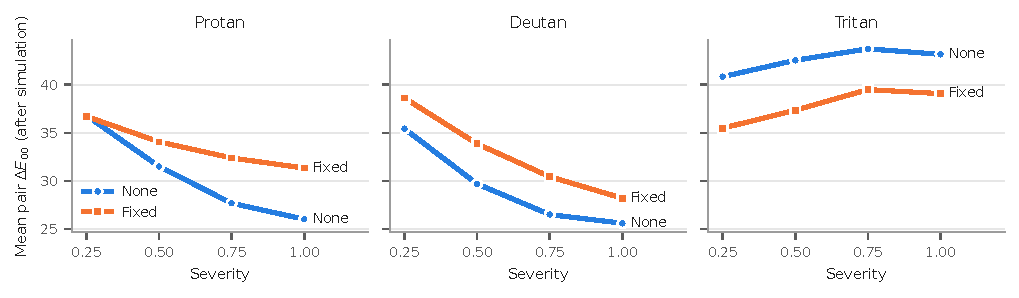
\includegraphics[width=\linewidth]{distinguishability_vs_severity}
  \caption{Mean pair distinguishability after CVD simulation as severity grows. Higher is
  better. Each line is one recoloring method.}
  \label{fig:severity}
\end{figure*}

\Cref{tab:recolor} and \cref{fig:severity} summarize the results. Without recoloring, pairs
lose distinguishability steadily as protan and deutan severity grows, falling to
\ResPairNoneProtanFull{} and \ResPairNoneDeutanFull{}~$\Delta E_{00}$ at full severity. The
fixed daltonization filter recovers part of that loss for red--green deficiencies:
\ResPairFixedProtanFull{} (protan) and \ResPairFixedDeutanFull{} (deutan) at full severity.
Across severities the deutan improvement is statistically reliable (median gain
\ResMedFixedDeutan~$\Delta E_{00}$, better on \ResImprovedFixedDeutan{} images,
$p_\mathrm{Holm}\ResPFixedDeutan$), while the protan gain is not
($p_\mathrm{Holm}\ResPFixedProtan$) because the filter changes little at low severity
(\cref{tab:paired}). For tritan the fixed filter is harmful: distinguishability drops from
\ResPairNoneTritan{} to \ResPairFixedTritan{}~$\Delta E_{00}$ (median
\ResMedFixedTritan, $p_\mathrm{Holm}\ResPFixedTritan$). A likely reason is that the Machado
tritan model shifts colors only slightly, so pairs remain well separated without help, while
the filter still moves them. The price of recoloring is a naturalness change of
\ResNatFixedDeutan--\ResNatFixedProtan~$\Delta E_{00}$ per pixel (\cref{fig:naturalness}).

\begin{table}[t]
  \centering
  \footnotesize
  \begin{tabular}{@{}llrrrr@{}}
\toprule
Method & Type & $n$ & Median $\Delta$ & Improved & $p_\mathrm{Holm}$ \\
\midrule
Fixed & Protan & 51 & +1.6 & 28/51 & 0.111 \\
Fixed & Deutan & 51 & +4.9 & 35/51 & 0.009 \\
Fixed & Tritan & 51 & -4.7 & 11/51 & \ensuremath{<}0.001 \\
\bottomrule
\end{tabular}

  \caption{Each method against no recoloring: per-image pair distinguishability (averaged
  over severities), two-sided Wilcoxon signed-rank tests with Holm correction. \emph{Improved}:
  images where the method raised distinguishability.}
  \label{tab:paired}
\end{table}

\begin{figure}[t]
  \centering
  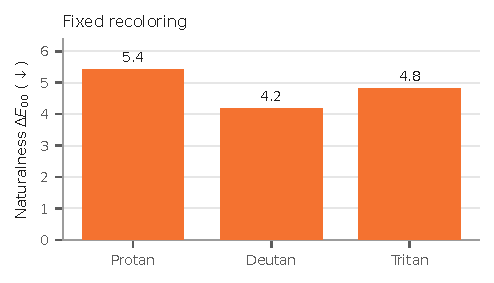
\includegraphics[width=\linewidth]{naturalness}
  \caption{Naturalness cost: mean per-pixel $\Delta E_{00}$ between the original and the
  recolored image for normal vision (lower is better). No recoloring is 0 by definition.}
  \label{fig:naturalness}
\end{figure}

\paragraph{By category.}
Gains depend on content (\cref{tab:category}). At full severity, averaged over CVD types,
natural scenes gain the most (\ResCatNoneNatural{} to \ResCatFixedNatural~$\Delta E_{00}$),
where red flowers and fruit sit on green foliage (\cref{fig:example}). Charts get slightly
worse (\ResCatNoneCharts{} to \ResCatFixedCharts), suggesting that when a chart's palette already
stays separable, the filter can push some series toward each other.

\begin{table}[t]
  \centering
  \footnotesize
  \begin{tabular}{@{}lcc@{}}
\toprule
Category & None & Fixed \\
\midrule
Charts & 27.9 & 25.2 \\
Maps & 33.4 & 33.1 \\
Traffic & 39.3 & 41.8 \\
Food & 29.5 & 31.4 \\
Coded items & 33.5 & 34.2 \\
Natural & 26.5 & 32.6 \\
\bottomrule
\end{tabular}

  \caption{Pair distinguishability ($\Delta E_{00}$) at severity 1.0 by category, averaged
  over CVD types.}
  \label{tab:category}
\end{table}

\begin{figure*}[t]
  \centering
  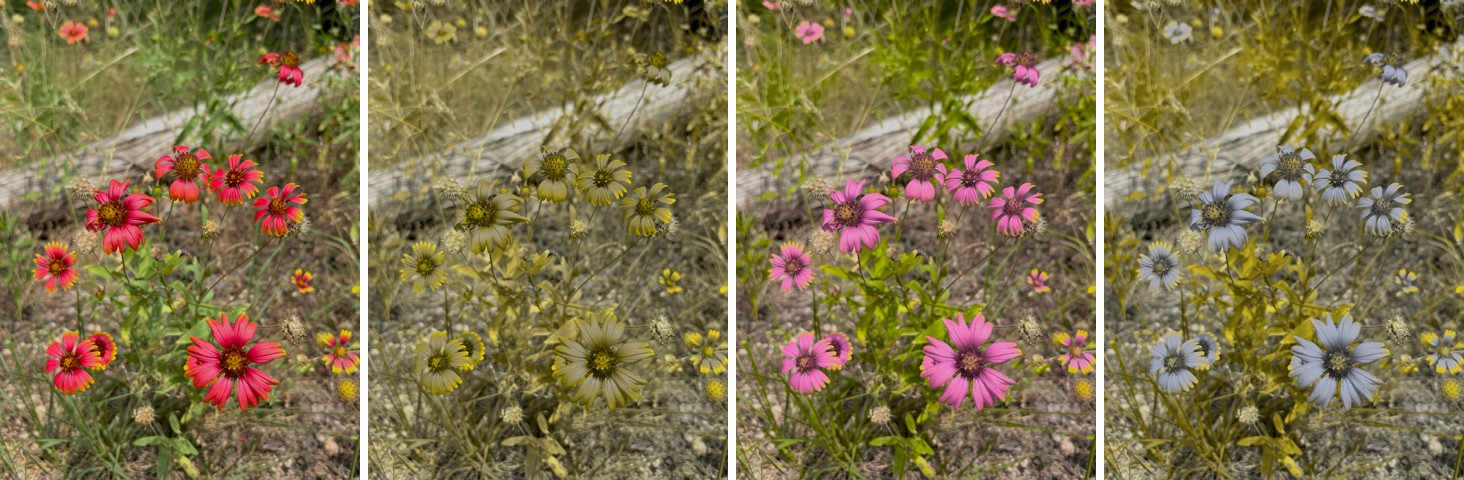
\includegraphics[width=\linewidth]{example.jpg}
  \caption{A team photograph (\ExampleImage). Left to right: original; deutan simulation
  (severity 1.0); fixed recoloring; deutan simulation of the recolored image. The red flowers
  that merge with the foliage under simulation become separable after recoloring.}
  \label{fig:example}
\end{figure*}

\ifdefined\ResPairPersonalizedDeutan
\paragraph{Personalized recoloring.}
With parameters tuned per type and severity on the tune split, personalized daltonization
reaches \ResPairPersonalizedDeutan{} (deutan) and \ResPairPersonalizedProtan{} (protan)
mean pair $\Delta E_{00}$, against \ResPairFixedDeutan{} and \ResPairFixedProtan{} for the
fixed filter, at a naturalness cost of \ResNatPersonalizedDeutan{} (deutan).
\TODO{Aliza: interpret once personalized results are in.}
\else
\paragraph{Personalized and neural recoloring.}
\TODO{Personalized and neural results appear here automatically: re-run run\_eval and
report\_assets once each method is available.}
\fi

\paragraph{Limitations.}
Distinguishability is measured on simulated vision, not on observers. The pairs were chosen to
be clearly different for normal vision, so the share below the JND is close to zero for every
method, and the metric reflects how much separation survives rather than whether pairs become
indistinguishable. Region means ignore texture and spatial context, and a single JND for all
pairs ignores region size.

\subsection{User study}
\label{sec:study}
Participants played the color-match game of \cref{sec:app}: each trial shows a test image with
two outlined regions from our annotations and asks which one answers a prompt such as ``which
apple is red?''. Each image appears under one recoloring condition per participant, rotated
across participants. For every participant and condition we compute accuracy and the median
response time of correct trials, then compare conditions with paired Wilcoxon signed-rank
tests~\cite{wilcoxon1945}, Holm-corrected~\cite{holm1979}, reporting the matched-pairs
rank-biserial correlation $r$~\cite{kerby2014} as effect size.

Each log records the CVD profile \emph{applied in the game}, not a diagnosis: normal-vision
players are given a simulated deutan profile (\cref{sec:app}), so they see the recolored image
through the deutan simulation. Their results therefore describe recoloring as seen through
simulated deutan vision, not by people with CVD. We report a separate subgroup only for
participants whose screening found a CVD, taken from the screening results rather than from
the logs.

\begin{table}[t]
  \centering
  \footnotesize
  \begin{tabular}{@{}lrrr@{}}
\toprule
Condition & Participants & Accuracy (\%) & Median RT (s) \\
\midrule
\multicolumn{4}{c}{\emph{No study sessions logged yet.}} \\
\bottomrule
\end{tabular}

  \caption{Mini-game results per condition (mean $\pm$ SD across participants; median of
  per-participant median response times on correct trials).}
  \label{tab:study}
\end{table}

\ifnum\StudyParticipants>0
\Cref{tab:study} summarizes \StudyTrials{} trials from \StudyParticipants{} participants.
\StudySimulatedParticipants{} of them played with a simulated CVD profile and
\StudyCvdParticipants{} were found to have a CVD by screening\ifnum\StudyCvdParticipants=0{},
so no result here describes observers with CVD\fi.
\TODO{Aliza: interpret the comparisons in results/study\_comparisons.csv.}
\else
\TODO{Study sessions have not been run yet; \cref{tab:study} fills in automatically from the
logs in results/study/ when \texttt{scripts/analyze\_study.py} is re-run.}
\fi

% Owner: whole team.
\section{Conclusion}
\label{sec:conclusion}
\TODO{Team: summary of findings, limitations from each section, and future work.}

{
    \small
    \bibliographystyle{ieeenat_fullname}
    \bibliography{refs}
}
\end{document}
